\section{Bitcoin}\label{sec:Bitcoin}
%%%%%%%%%%%%%%%%%%%%%%%%%%%
% *** FIRST SUB-SECTION ***
%%%%%%%%%%%%%%%%%%%%%%%%%%%
\subsection{Introduction}

Bitcoin it's the first fully decentralized cryptocurrency. It was invented by
Satoshi Nakamoto in 2008 and it was the first real implementation of Blockchain.
Bitcoin can be either defined as a protocol, a digital currency and a platform.

Bitcoin can be seen as a combination of
\vspace{-\topsep}
\begin{itemize}
  \item[-] a decentralized peer-to-peer-network (the Bitcoin protocol)
  \item[-] a public transaction ledger (the blockchain)
  \item[-] a set of rules for validating transactions (consensus rules)
  \item[-] a mechanism for reaching distributed consensus on the blockchain (distributed
  consensus algorithm)
\end{itemize}
\vspace{-\topsep}
that allows the usage of the digital currency named bitcoin.

From now on, Bitcoin with the capital $B$ will refer to the Bitcoin protocol
while bitcoin with the lowercase $b$ will refer to the bitcoin currency.



Bitcoin is a distributed peer-to-peer system in which users can exchange
currency over the network just as it can be done with conventional currency.
However, unlike traditional currencies, bitcoins are enterely virtual and thus
there are no physical coins. In particular, there are not even virtual coins since
they are implied in the transactions that send value from a sender to a receiver:
users have private keys which allow them to prove the ownership of bitcoins and
sign transactions in order to unlock the value and transfer it to another user.
These keys are the only requirement for spending bitcoins and therefore they are
protected in wallets stored in the user's devices.

\subsubsection*{The reference implementation}
Bitcoin is an open source project and is developed by a community of volunteers.
The first implementation was released by Satoshi Nakamato in 2008 (the only member
of the development community at the time). That implementation during the years
has been heavily modified and improved evolving into what is known as \emph{Bitcoin
Core}, which is now the reference implementation of the Bitcoin system. This
implementation is considered the authoritative one and it specifies how each
part of the system has to be implemented.














%%%%%%%%%%%%%%%%%%%%%%%%%%%
% *** SECOND SUB-SECTION ***
%%%%%%%%%%%%%%%%%%%%%%%%%%%
\subsection{Keys and Addresses}
As mentioned in this chapter's introduction, ownership of bitcoin is established
through digital keys, bitcoin addresses, and digital signatures.

In order to be included in the Bitcoin blockchain, transactions require a valid
signature which can be generated only with a private (secret) key. The private
key therefore proves the ownership of bitcoins by signing transactions and
transferrig value from a user to another. Keys come in pairs consisting of a
private (secret) key and a public key and they are generated through Elliptic
Curve Cryptography. In analogy with the traditional banking,the public key can be
seen as the bank account number while the private key as the secret PIN (or the
signature on a check) which provides control over the account by allowing to unlock
the value and transferring it to other people.

\subsubsection{Adresses}
An address is unique string of digits and characters which identify the originator
and/or the destination of a transaction. Addresses are derived from public keys
through one-way cryptographic hashing in order to obtain the public key fingerprint.
In particular, a Bitcoin address is derived by hashing the user's public key it twice,
first with the SHA-256 algorithm and then with RIPEMD160. This produces a 160-bit
hash, which is then prefixed with a version number and finally encoded using
Base58Check encoding. The final result is a 26-35 chatacters string which begins
with 1 (public key address) or 3 (pay-to-script-hash address) and it looks like the
the string below:
\begin{center}
  \texttt{1J7mdg5rbQyUHENYdx39WVWK7fsLpEoXZy}
\end{center}
The generation process scheme is shown in figure \ref{fig:address-generation}.

\begin{figure}[!htb]
	\centering
	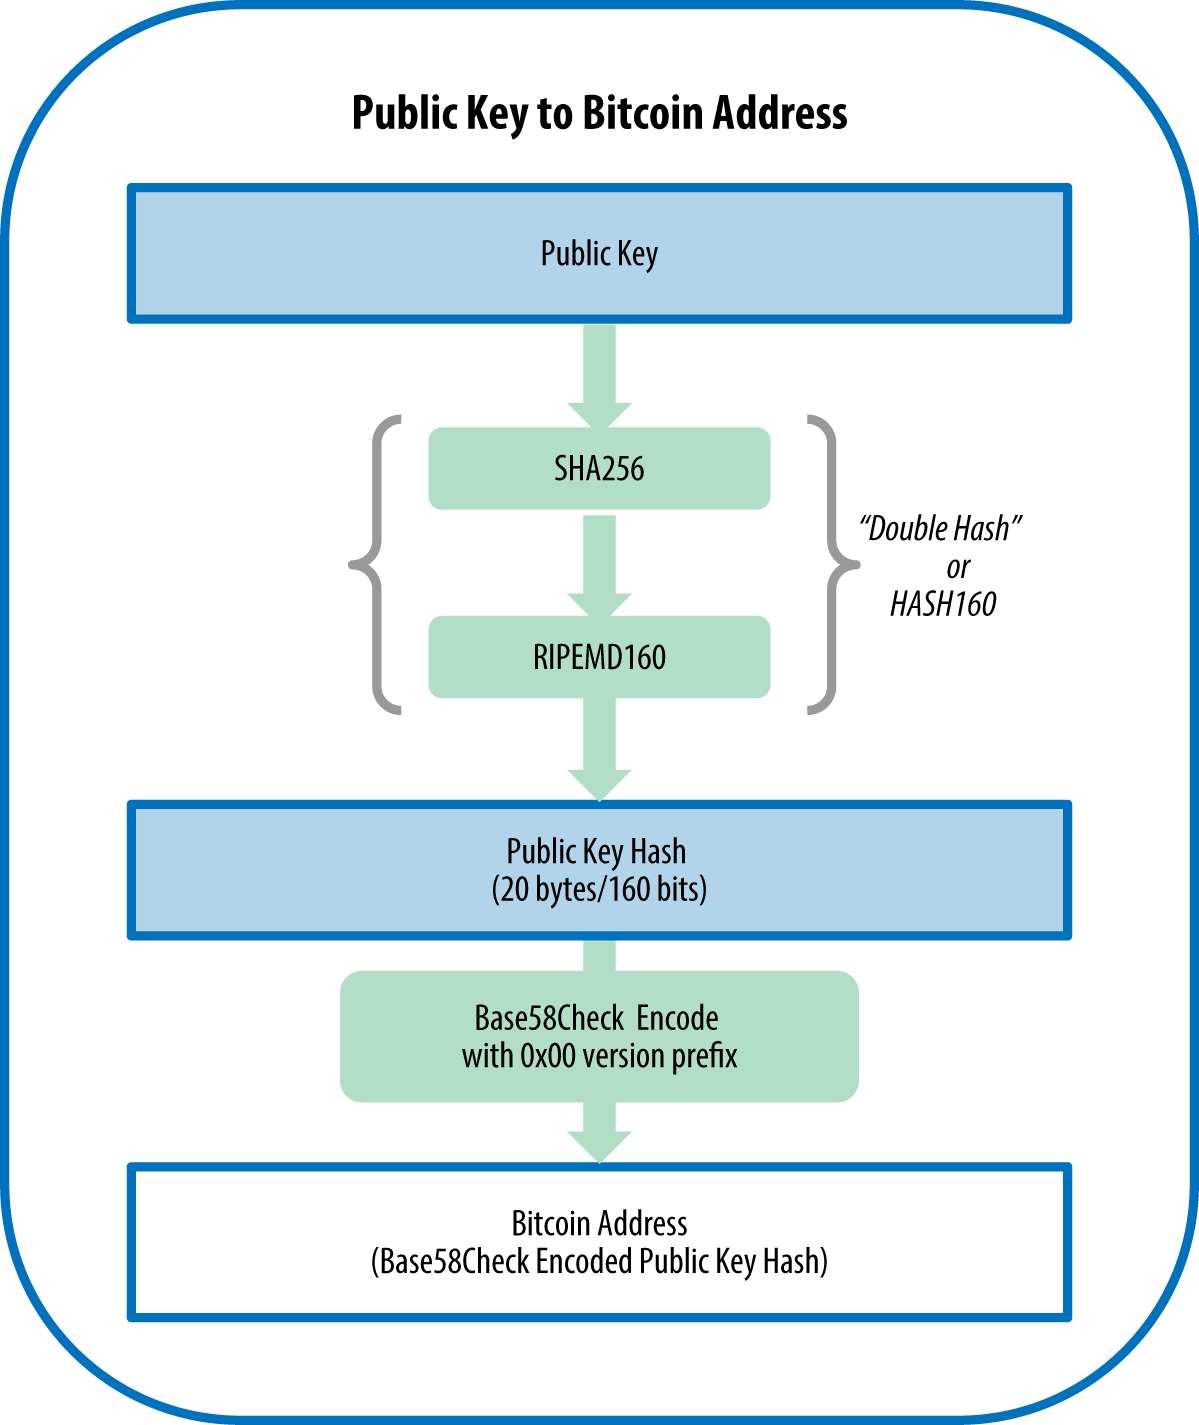
\includegraphics[width=0.85\linewidth]{img/address-generation.png}
	\caption{Bitcoin address generation scheme}
	\label{fig:address-generation}
\end{figure}

\paragraph{Base58 and Base58Check} Base58 is an encoding scheme which allows to
represent long numbers as alphanumeric strings. It is a subset of Base64, which
represent numbers using 26 lowercase letters, 26 capital letters, 10 numerals,
and 2 more ``special'' characters and it's usually used to encode email
attachments. In particular, Base58 is Base64 without all that characters that
are frequently mistaken for one another, namely it is Base64 without the 0
(number zero), O (capital o), l (lower L), I (capital i) and the two special
characters. Base58Check is a Base58 encoding with an additional checksum of four
bytes added to the end of the data that is being encoded which prevents a
mistyped bitcoin address from being accepted by the wallet software as a valid
destination.


\paragraph{P2SH and P2PKH}  As already mentioned before, Bitcoin addresses that
begin with the number ``$3$'' are pay-to-script hash (P2SH) addresses. Unlike
the address which start with ``$1$'', also known as pay-to-public-key-hash
(P2PKH), which are associated to a public key owned by a user, the P2SH
addresses designate the beneficiary of a Bitcoin transaction as the hash of a
script. When a user send a bitcoin to a P2PKH address, that bitcoin can only
be spent by the receiver by presenting the corresponding private key signature
and public key hash associated to its address. When instead the bitcoin is sent to
a P2SH address, namely to the hash of a script, the requirements for spending that
bitcoin are defined by the script and are usually more restrictive (for example it
could be required more than one signature to prove the ownership). A P2SH address
is derived from a transaction script in the same way a P2PKH address is derived
from a public key (double hashing + Base58Check encoding).


\subsubsection{Keys}
Public and private keys in Bitcoin are generated through ECC and they can be
represented in different formats. All the possible representations, even if they
look different, correspond to the same number. This has been done in order to
facilitate people to read and transcribe the keys without introducing errors.

\paragraph{Private keys}
Private keys are simply a 256-bit random number. For generating it, Bitcoin
software uses the underlying operating system’s random number generators which
usually is initialized by a human source of randomness, like for example the elapsed
time between the pression of the keys of the keyboard.

\paragraph{Private key formats}
The private key can be represented in different formats (shown in table
\ref{tab:private-key-formats}), each one corresponding to the same 256-bit number.
Different formats are used in different circumstances: for example Hexadecimal
and raw binary formats are used internally in software while WIF is used by users.
\begin{table}[h!]
\centering
\resizebox{\textwidth}{!}{%
\begin{tabular}{@{}lll@{}}
\toprule
\multicolumn{1}{c}{\textbf{Type}} & \multicolumn{1}{c}{\textbf{Prefix}} & \multicolumn{1}{c}{\textbf{Description}}                                     \\ \midrule
Raw                               & None                                & 32 bytes                                                                     \\
Hex                               & None                                & 64 hexadecimal digits                                                        \\
WIF                               & 5                                   & Base58Check encoding \\
WIF-compressed                    & K or L                              & As above, with added suffix 0x01 before encoding                             \\ \bottomrule
\end{tabular}%
}
\caption{Private key representation formats \cite{antonopoulos2017mastering}}
\label{tab:private-key-formats}
\end{table}

\paragraph{Public key generation}
Public keys are generated starting from the private keys using elliptic curve
multiplication, which is a so-called ``trap door'' function: it is easy to do in
one direction (multiplication) and impossible to do in the reverse direction (division).
Bitcoin uses the elliptic curve and the set of constants specified by the secp256k1
standard, defined by the NIST. The elliptic curve used is defined by the following
equation:
\begin{equation}\label{eq:bitcoin-curve}
  y^2 = (x^3 + 7)~\text{over}~(\mathbb{F}_p)
\end{equation}
\begin{center}
  or, equivalently:
\end{center}
\begin{equation}
  y^2 \bmod p = (x^3 + 7) \bmod p
\end{equation}
where $p = 2^{256} – 2^{32} – 2^9 – 2^8 – 2^7 – 2^6 – 2^4 – 1$ is a very large prime number.
Starting from the private key $k$, the public key $K$ is calculated multiplying
it by a predetermined point on the curve called the generator point $G$ (defined
by the secp256k1 standard) in order to produce another point somewhere else on
the curve, which will correspond to the public key $K$:
\[K = k * G\]
Since the generator point $G$ is always the same for all bitcoin users, a
private key $k$ multiplied with $G$ will always result in the same public key $K$.
The relationship between $k$ and $K$ is fixed and known but it can only be
calculated in one direction (from $k$ to $K$), so it's impossible to derive from
an address (derived from K) the corresponding user's private key.

\paragraph{Public key formats} In Bitcoin, since ECC is used, a public key in
the uncompressed format is a point on an elliptic curve consisting of the
coordinates pair $(x,y)$. Uncompressed public keys are presented with the prefix
\code{04} followed by two 256-bit numbers, one for each coordinate, and
therefore they are 65 Bytes long. The compress format instead includes only the
x-coordiante since the y one can be derived from it and by solving the equation
\eqref{eq:bitcoin-curve} it uses the prefixes \code{03}, if the y-coordinate is an
odd number, or \code{02}, if it is an even number. The length of a compressed
public key is therefore 33 Bytes. Compressed public keys were introduced in
order to reduce the size of the transactions, since the most of them also include
the public key. The reason why two different prefixes are required for
compressed keys is that the left side of the equation \eqref{eq:bitcoin-curve} is
$y^2$ and therefore the solution for $y$ is a square root, which can have a
``positive'' or ``negative value'': graphically, this means that the
y-coordiante can either be above or below the x-axis and therefore two different
points can be identied since the curve is symmetric. Actually since we are in
fhe field $\mathbb{F}_p$ it doesn't make sense talking about positive and
negative values: the y-coordinate can in fact be \emph{even} or \emph{odd}
(which correspond to the positive/negative terms used before).

Note that a a public key in both compressed and uncompressed formats always
corresponds to the same private key, even if the two formats have a different
representation. The address derived from the compressed public key however is
different from the address derived from the uncompressed one. To solve this
issue, compressed private keys have been introduced: a compressed private key is
a ``private key from which only compressed public keys should be derived'',
while uncompressed private keys are ``private keys from which only uncompressed
public keys should be derived'' \cite{antonopoulos2017mastering}.
